\chapter{Verification\label{cha:chapter5}}
This chapter discusses the verification carried out to ensure proper working of our code. The results for the same will be discussed in Results and Discussion \ref{cha:chapter5}.

\section{Heat Transfer Verification in One Dimensional Settings for the Enthalpy Problem}
To verify the temperature distribution obtained from the numerical scheme, we compare the results obtained from the numerical scheme to the analytical one. We assume a one dimensional bar of unit length. We have considered two different types of boundary conditions, in order to verify the temperature distribution.\\

\noindent \textbf{A) Specified Temperature Boundary Condition (Type I BC): -}\\
 A boundary condition where both the ends of the bar are held at a constant fixed temperature is commonly referred to as specified temperature boundary condition\cite{Cengel_Ghajar_2020}. We assume, both the ends of the rod are at fixed 0 dimensionless temperature and $T_{initial} = f(x)$ as the initial temperature distribution, this means that our material is in liquid phase and there is no phase change. Mathematically we can write: -
 \begin{subequations}
     \begin{align}
         T(x,0) = T_{initial} = -\frac{1}{2}sin(3\pi x)+\frac{3}{2}sin(\pi x) \label{eq:type1initialBCS} \\ \nonumber
         \\
         T(0,t) \ = \ 0 \quad \text{and} \quad T(1,0) \ = \ 0 \label{eq:type1BCS}
     \end{align}
 \end{subequations}
 Figure \ref{fig:Type1_BC} depicts our setup for the heat transfer verification.\\
 The analytical solution for equation \eqref{eq:nondimensional} subject to initial \eqref{eq:type1initialBCS} and boundary \eqref{eq:type1BCS} conditions is given by equation \eqref{eq:AnalyticalBCS}\cite{Hancock}.
 \begin{subequations}
     \begin{align}
         T_{(x,t)} = \frac{3}{2}sin(\pi x)e^{-\pi^2 t}-\frac{1}{2}sin(3\pi x)e^{-9\pi^2 t} \label{eq:AnalyticalBCS}
     \end{align}
 \end{subequations}
 \begin{figure}[htb]
  \centering
  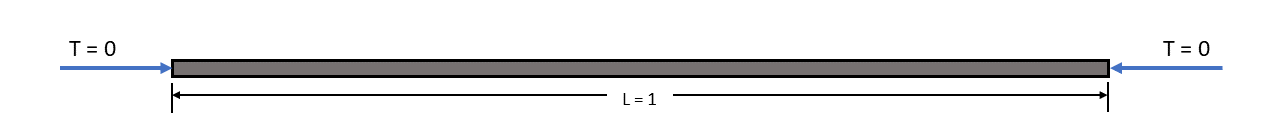
\includegraphics[width=11cm]{Type1_BC.png}\\
  \caption{Setup for the Heat Transfer Verification with type 1 boundary condition}
  \label{fig:Type1_BC}
\end{figure}\\
\noindent \textbf{B) Specified Heat Flux Boundary Condition (Type II BC): -}\\
A boundary condition where heat flux is specified at one end and the other end is assumed to be fixed at a dimensionless temperature is known as specified heat flux boundary condition\cite{Cengel_Ghajar_2020}. In our case, we  assume that the end x = 0 is insulated $\left(\frac{\partial T}{\partial x} =  0 \right)$, where as the other end x = 1 is at a fixed 0 dimensionless temperature ($T_{1,t} = $ 0) with $T_{initial} = T_{x,0}$ = 1 as the initial temperature distribution. The figure \ref{fig:Temperature_Distribution} shows the setup.  
\begin{figure}[htb]
  \centering
  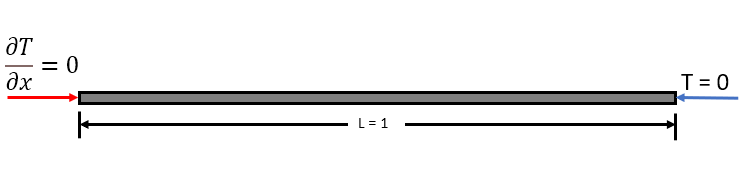
\includegraphics[width=9cm]{Testing.png}\\
  \caption{Setup for the Temperature Distribution Verification}
  \label{fig:Temperature_Distribution}
\end{figure}
The equation \eqref{eq:Analytical_Solution} \cite{Hancock}is the analytical solution to the temperature distribution over time for the equation \eqref{eq:nondimensional} subject to type 2 boundary condition.\\
\begin{subequations}
\begin{align}
    T(x,t) = \frac{4 T_{initial}}{\pi} \sum_{n=1}^{\infty} \frac{(-1)^{n+1}}{2n-1}cos \left ( \frac{2n-1}{2} \pi x \right) exp  \left (- \frac{(2n-1)^2 \pi^2}{4}t\right)\label{eq:Analytical_Solution}
\end{align}
\end{subequations}\\
where: -\\
\indent $T_{initial}$ = Constant Initial Temperature Distribution\\
\indent $t$ = Time\\
We have carried out the verification of the position of the interface for the one dimensional Stefan problem approach in the next chapter. 